\documentclass[11pt]{beamer}

%\usetheme{Warsaw}
%\usetheme{Antibes}
%\usetheme{Szeged}
%\usetheme{Szeged}
\usetheme{Montpellier}

\usecolortheme{orchid}

\usepackage[utf8]{inputenc}
\usepackage[english]{babel}
\usepackage{amsmath}
\usepackage{amsfonts}
\usepackage{amssymb}
\usepackage{graphicx}
\author{SIE doctoral school}
\title{An introduction to Beamer}
%\setbeamercovered{transparent} 
\setbeamertemplate{navigation symbols}{} 
%\logo{} 
\institute{Université Savoie Mont Blanc} 
%\date{} 
\subject{Introduction to \LaTeX} 
\begin{document}


\section{Introduction}

\begin{frame}[plain] % PLAIN = EMPTY FRAME
    \titlepage
\end{frame}

\begin{frame}
    \tableofcontents
\end{frame}

\section{Basic frames}


\subsection{Blocks}

% FRAME 1
\begin{frame}{Blocks (1/2)}
    \begin{center}
        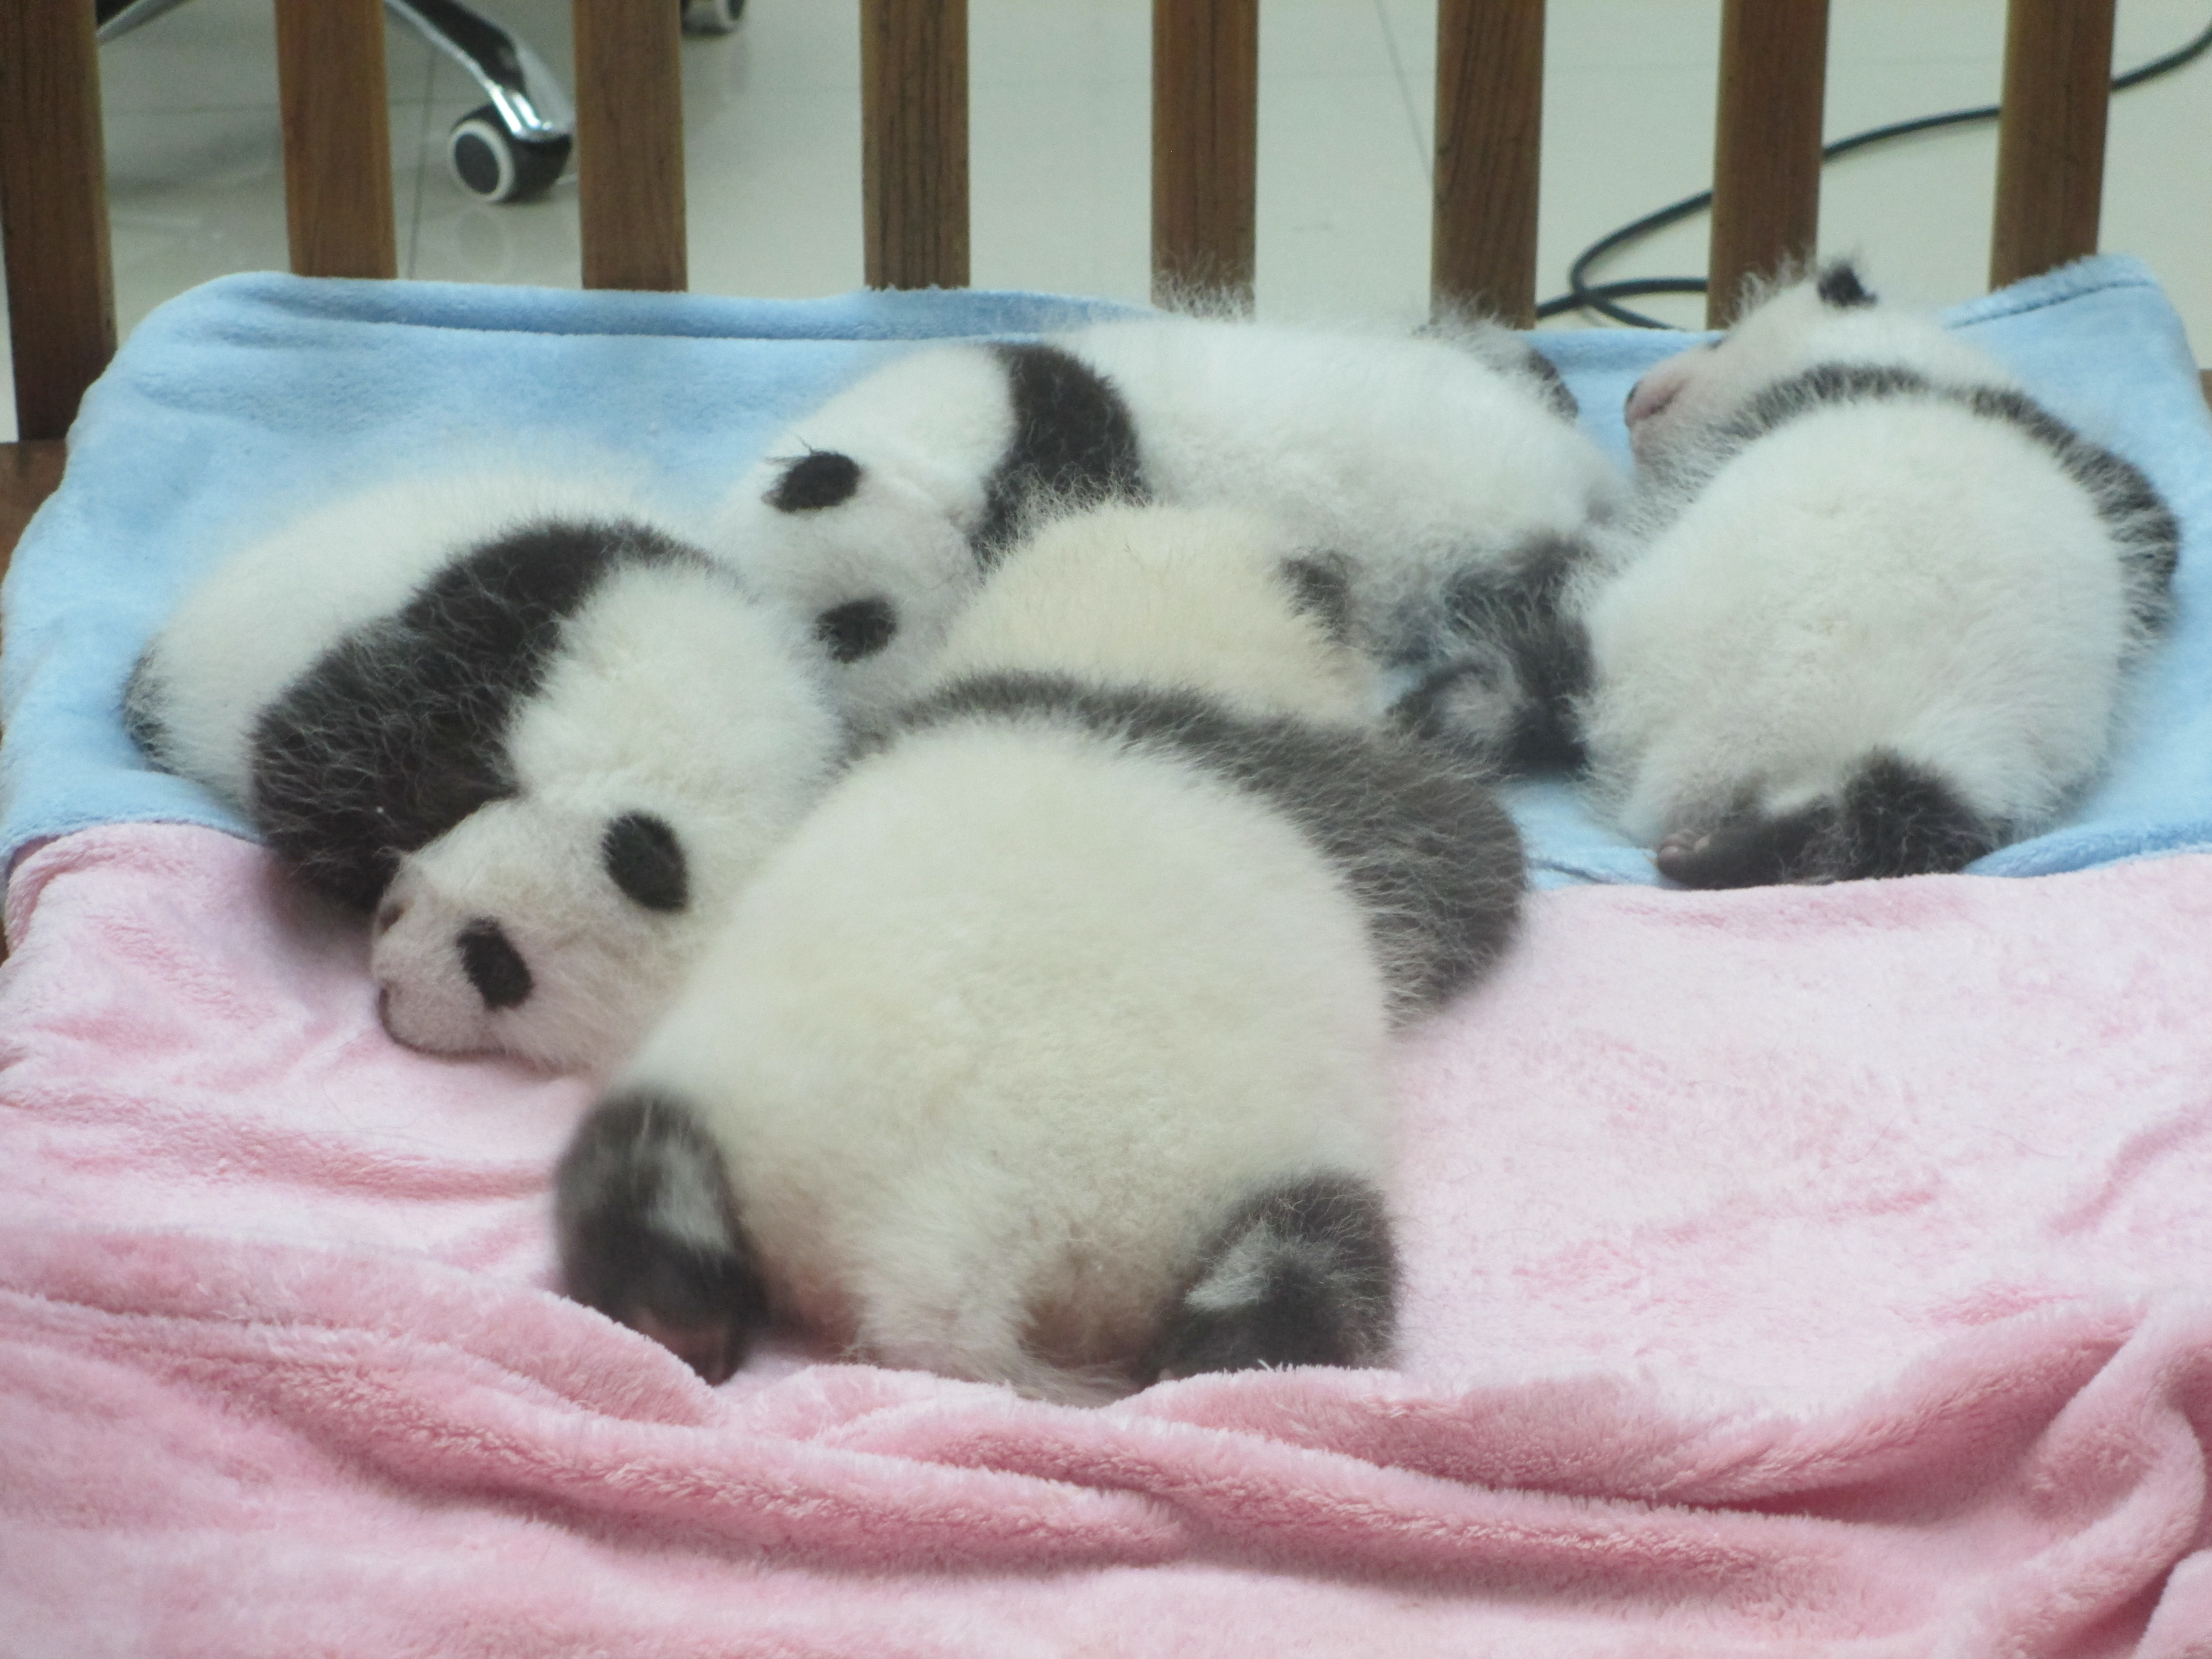
\includegraphics[width = .55\textwidth]{../figures/panda_puppies}
    \end{center}

    \begin{block}{A standard block}
        \begin{itemize}
            \item Some data.
            \item Some other data.
        \end{itemize}
    \end{block}
\end{frame}


% FRAME 2
\begin{frame}{Blocks (2/2)}
    \begin{center}
        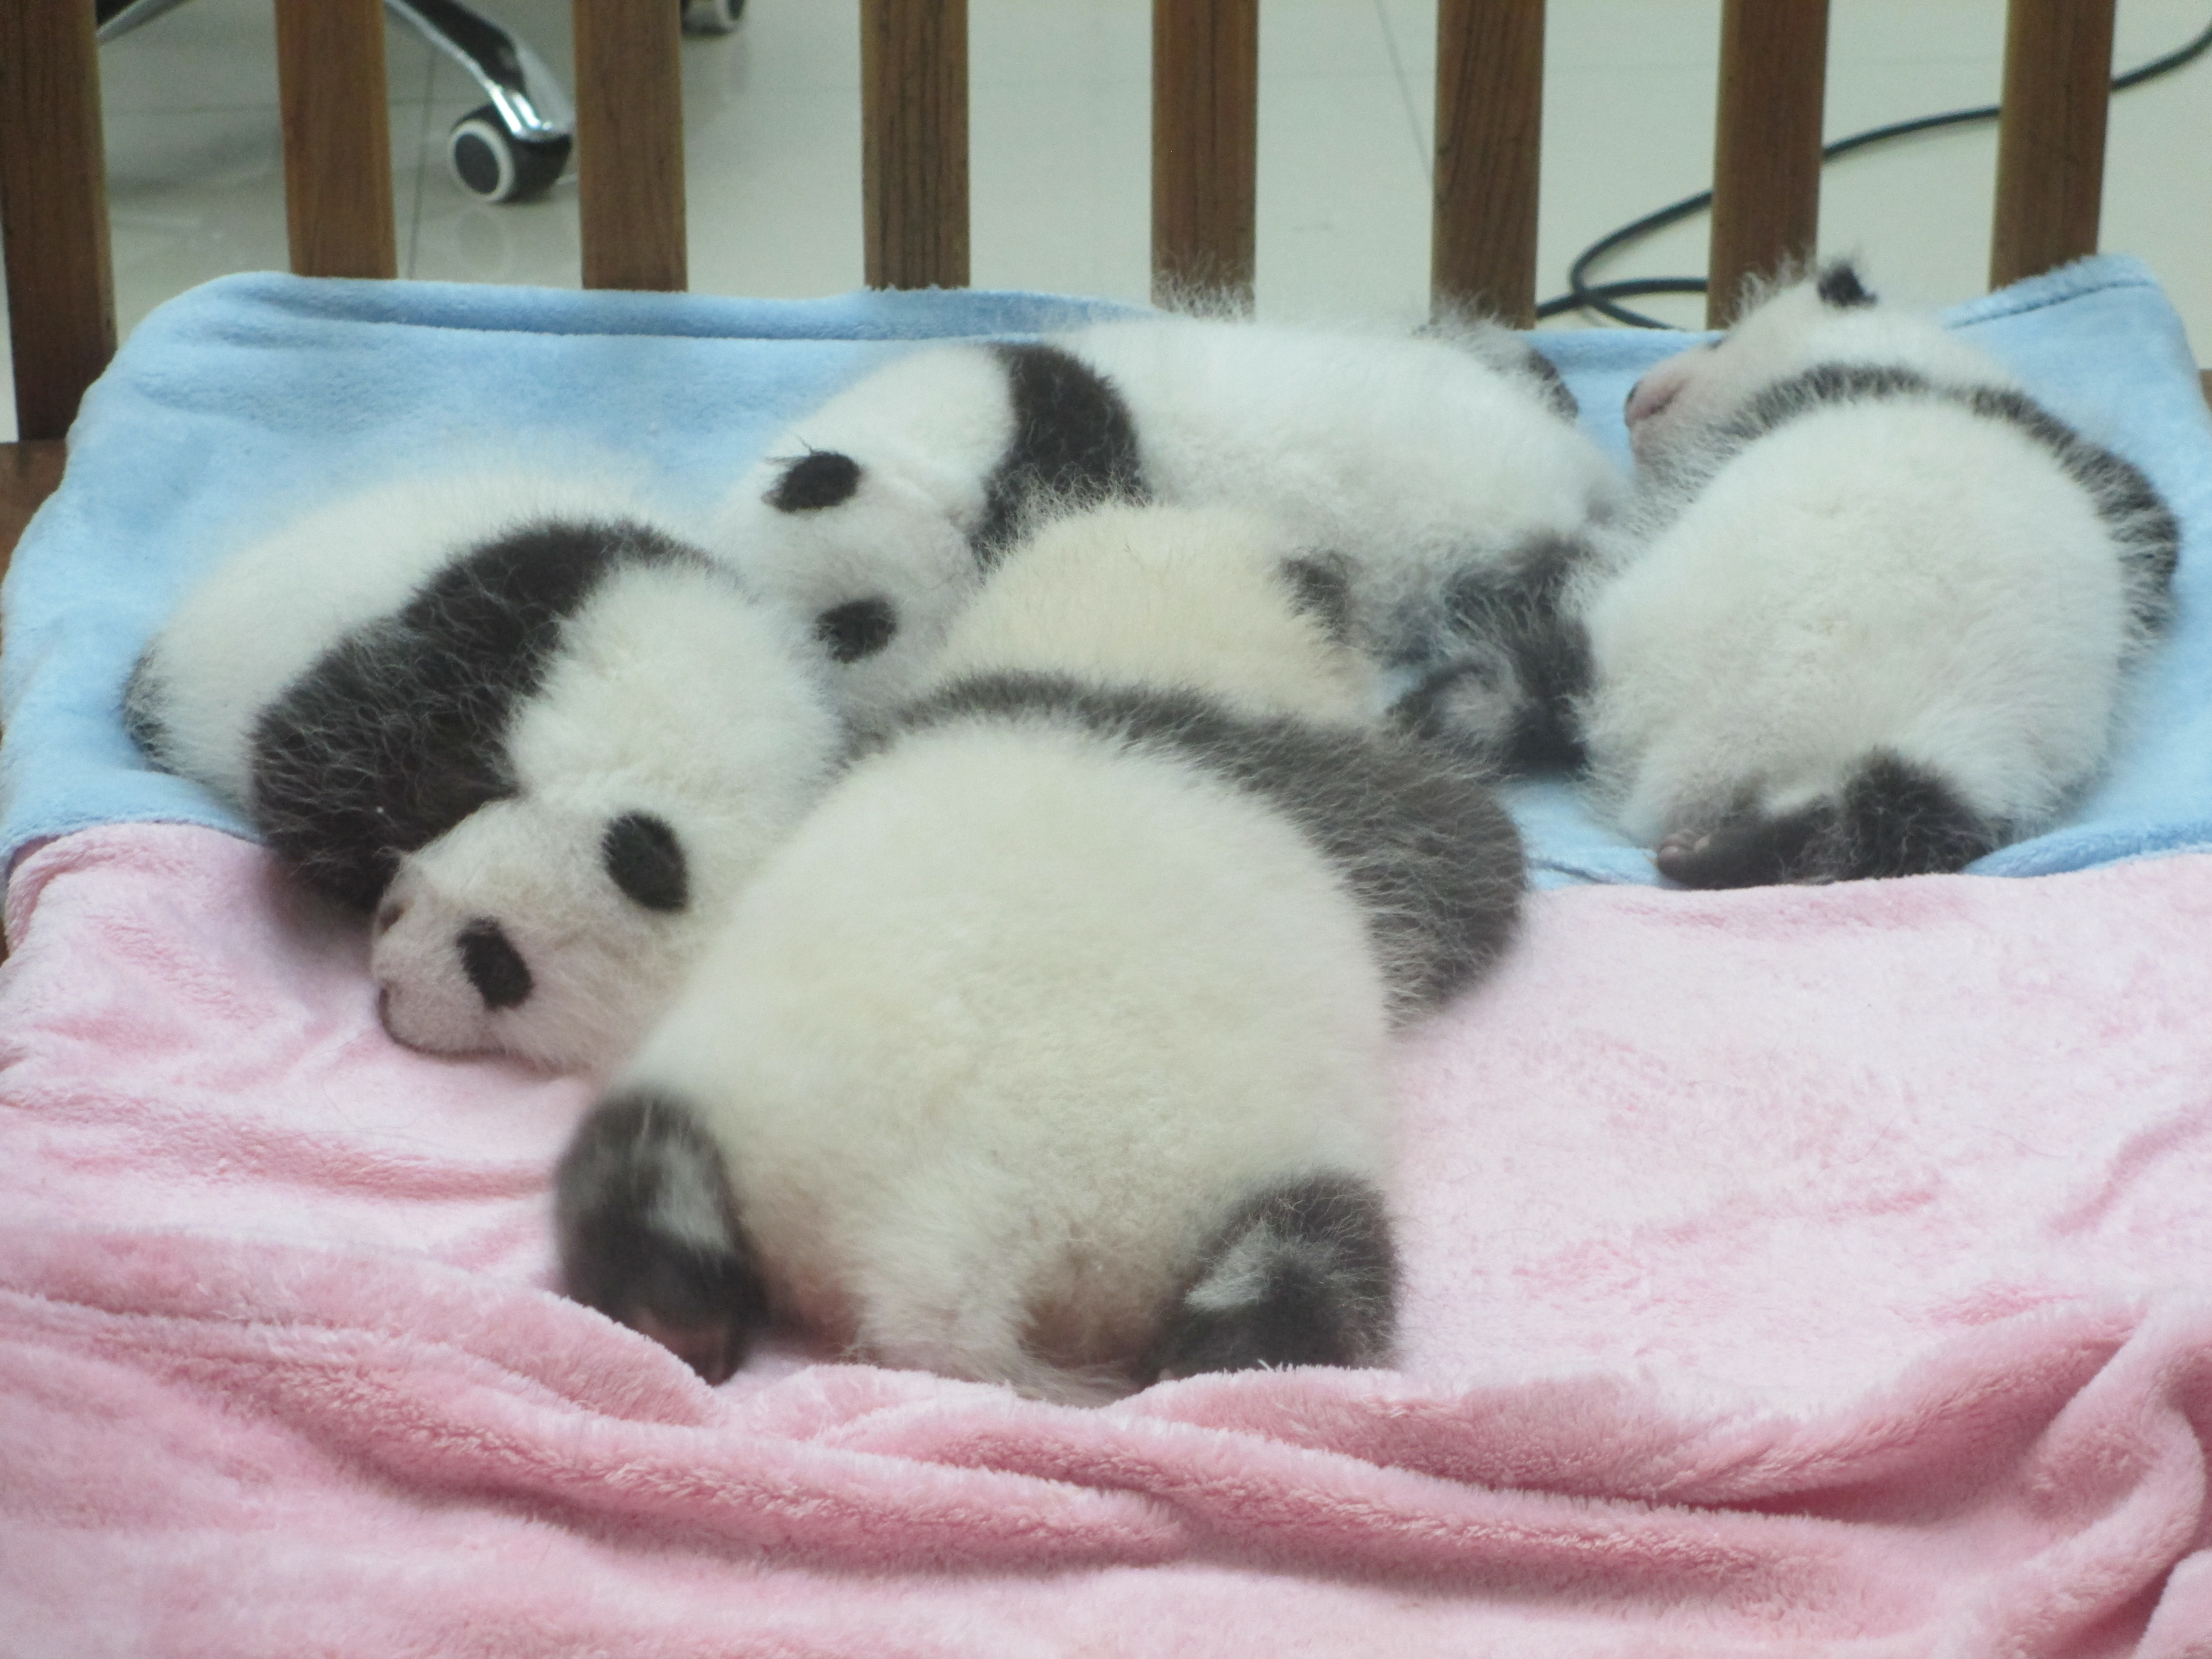
\includegraphics[width = .55\textwidth]{../figures/panda_puppies}
    \end{center}

    \begin{alertblock}{An alertblock}
        \begin{itemize}
            \item Some data.
            \item Some other data.
        \end{itemize}
    \end{alertblock}
\end{frame}

\subsection{Frames with columns}
\begin{frame}{Frames with columns}
    \begin{columns}[c] % c = Vertical centering
        \column{.6\textwidth}
        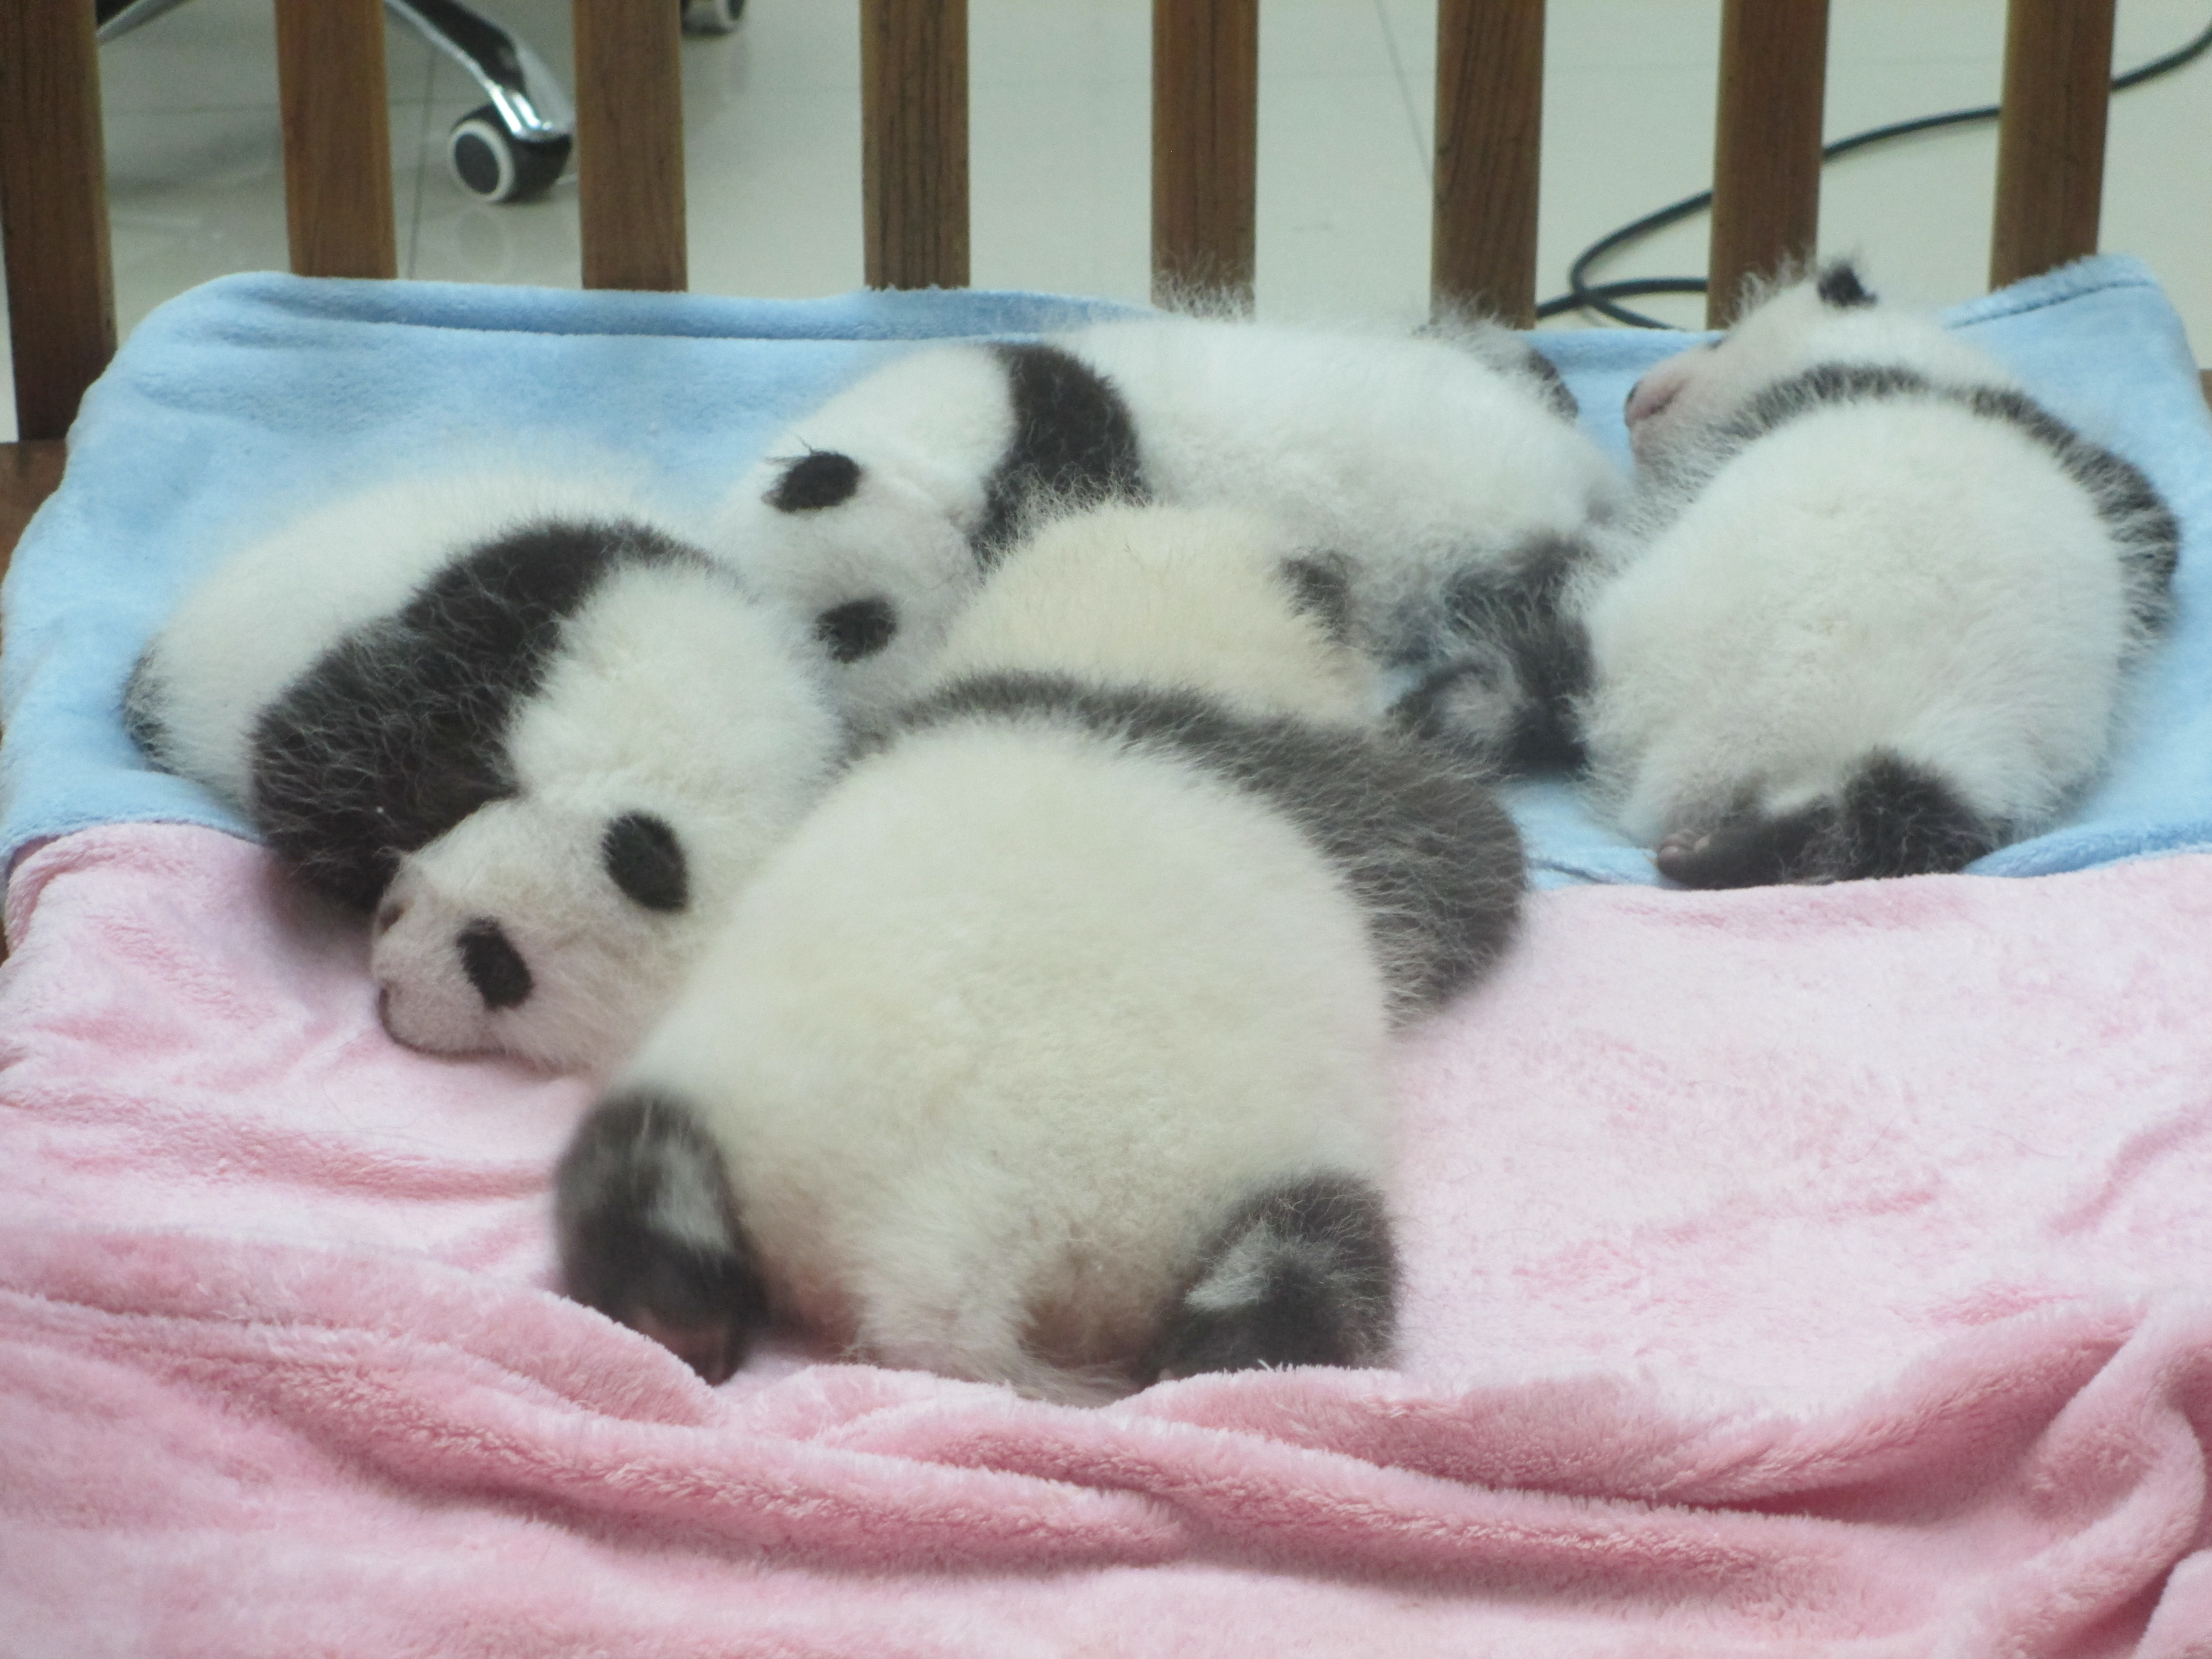
\includegraphics[width = 1.\textwidth]{../figures/panda_puppies}
        \column{.4\textwidth}
        \begin{block}{A standard block}
            \begin{itemize}
                \item Some data.
                \item Some other data.
            \end{itemize}
        \end{block}

        \begin{alertblock}{An alertblock}
            \begin{itemize}
                \item Some data.
                \item Some other data.
            \end{itemize}
        \end{alertblock}
    \end{columns}
\end{frame}

\section{Overlays}

\subsection{Basic overlays}

\begin{frame}{Overlays }

    \begin{overprint}
        \onslide<1> 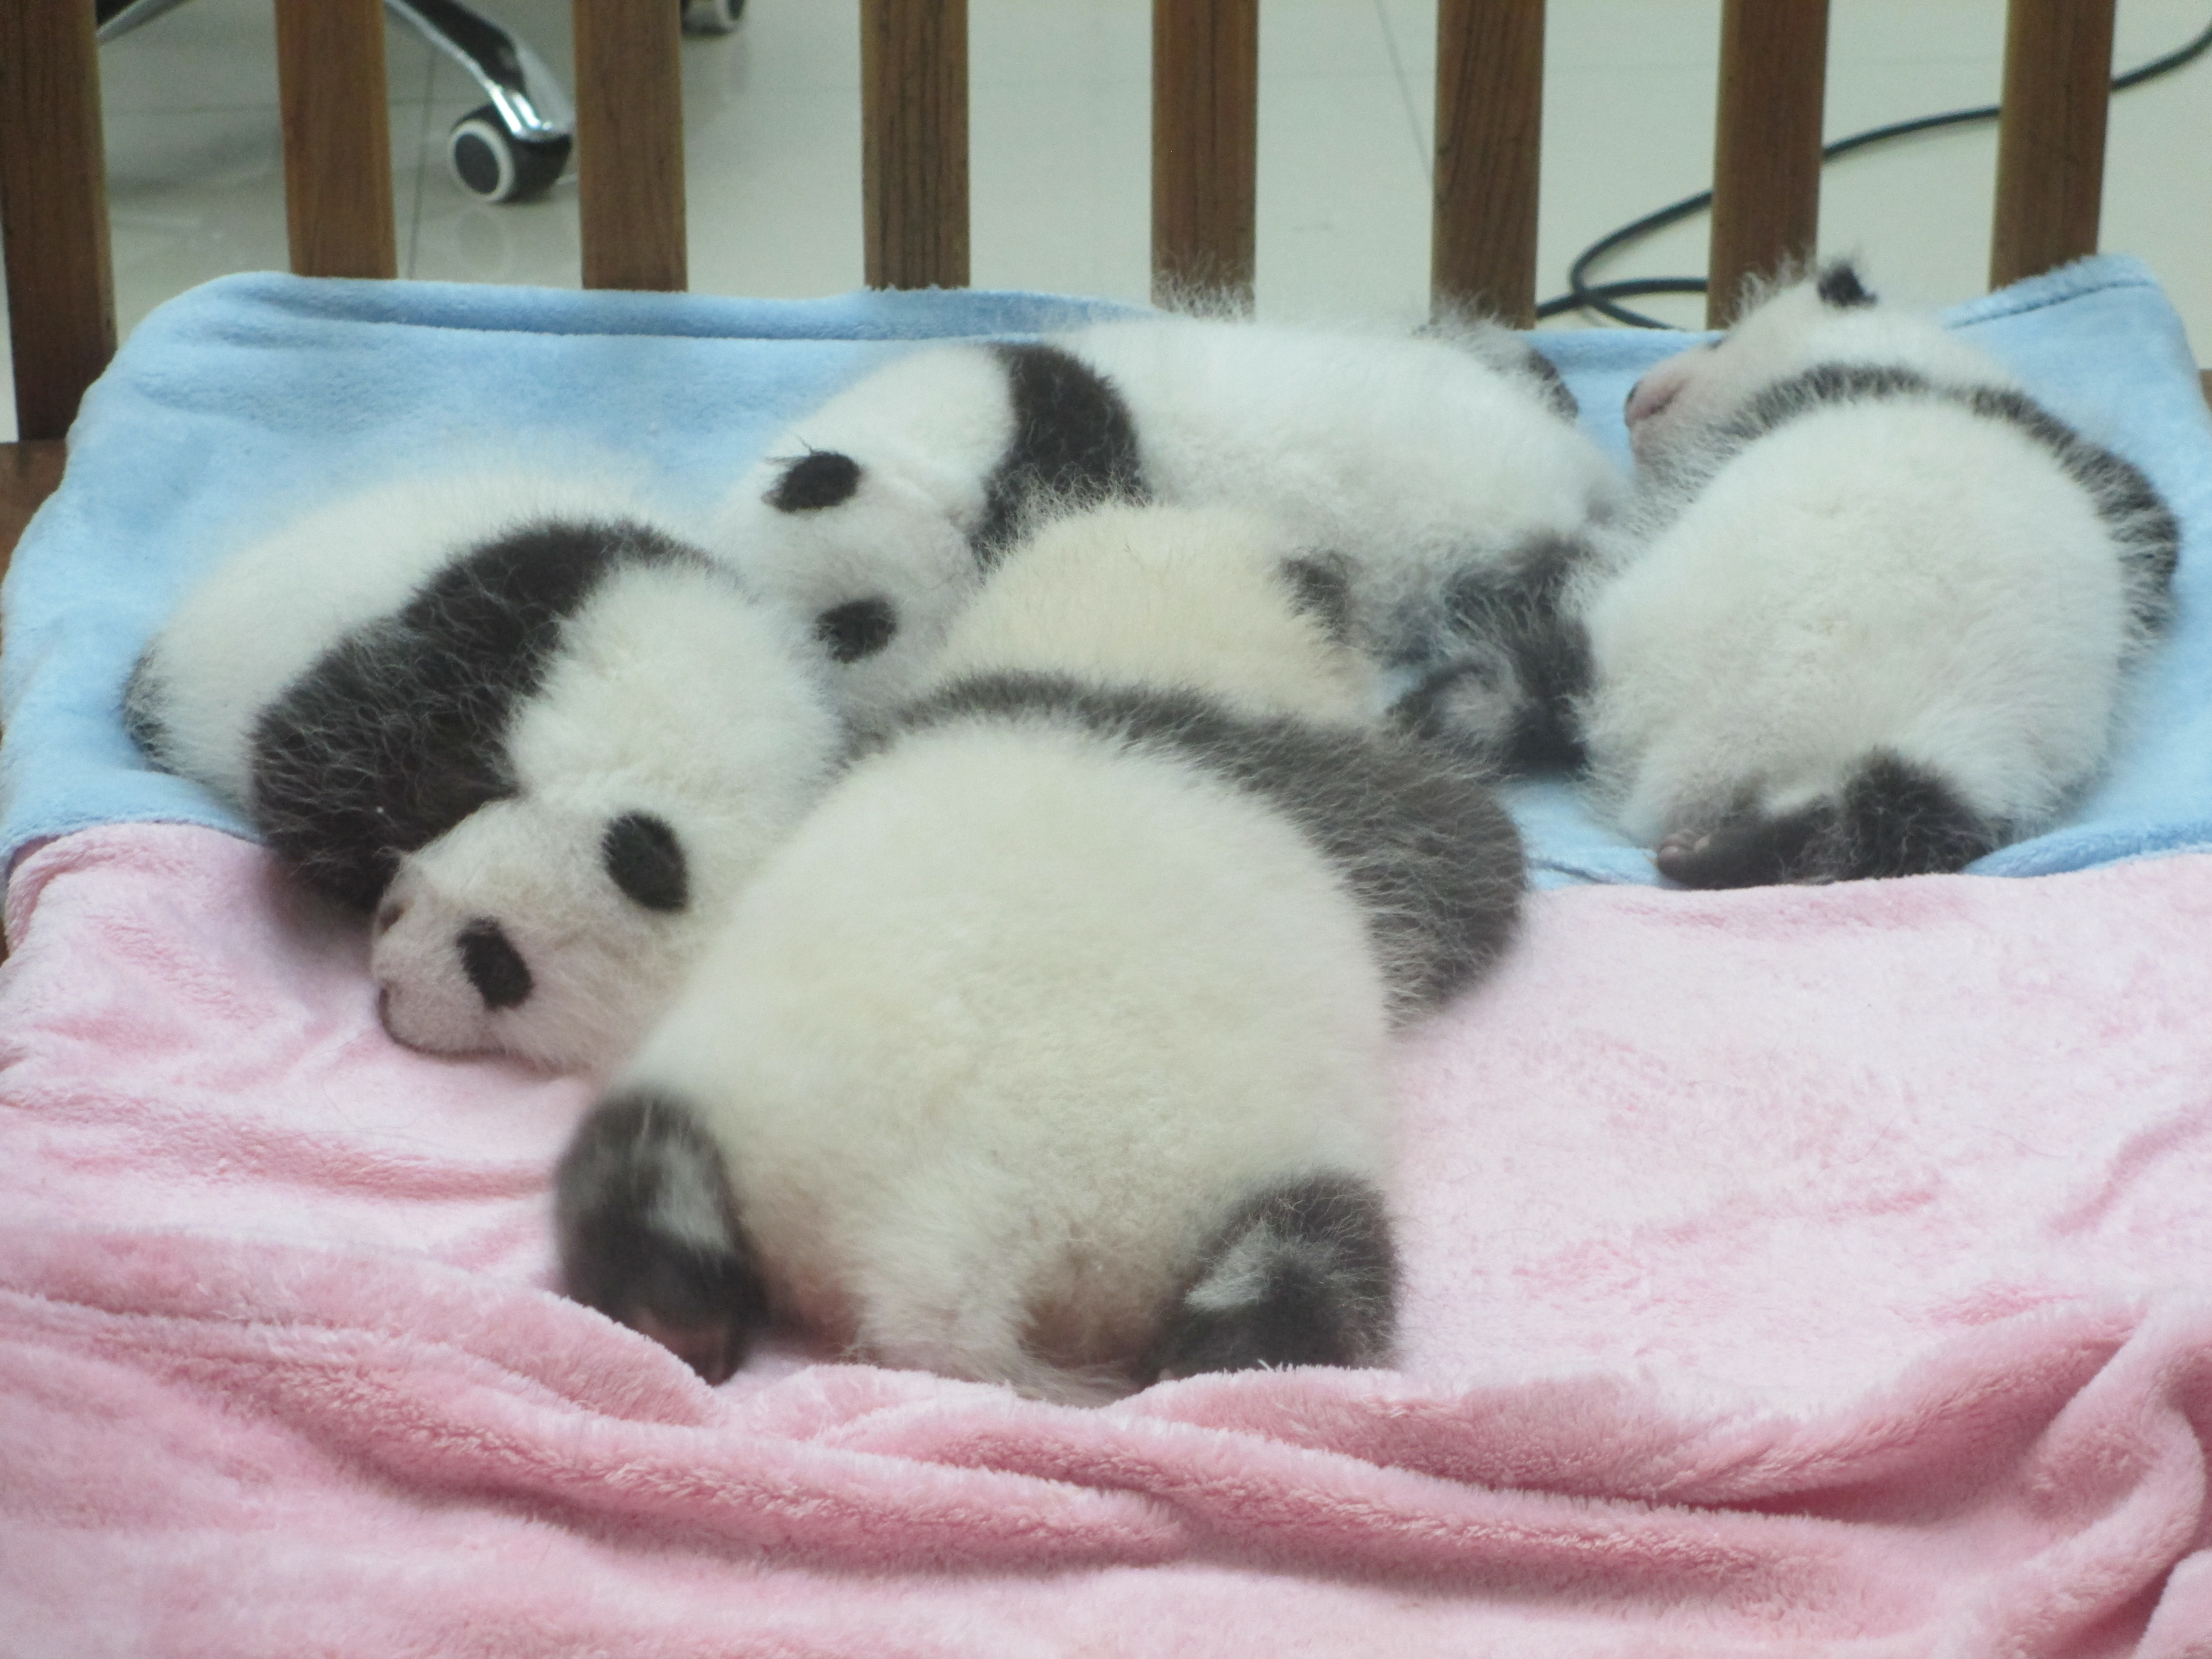
\includegraphics[width = .55\textwidth]{../figures/panda_puppies}
        \onslide<2-> 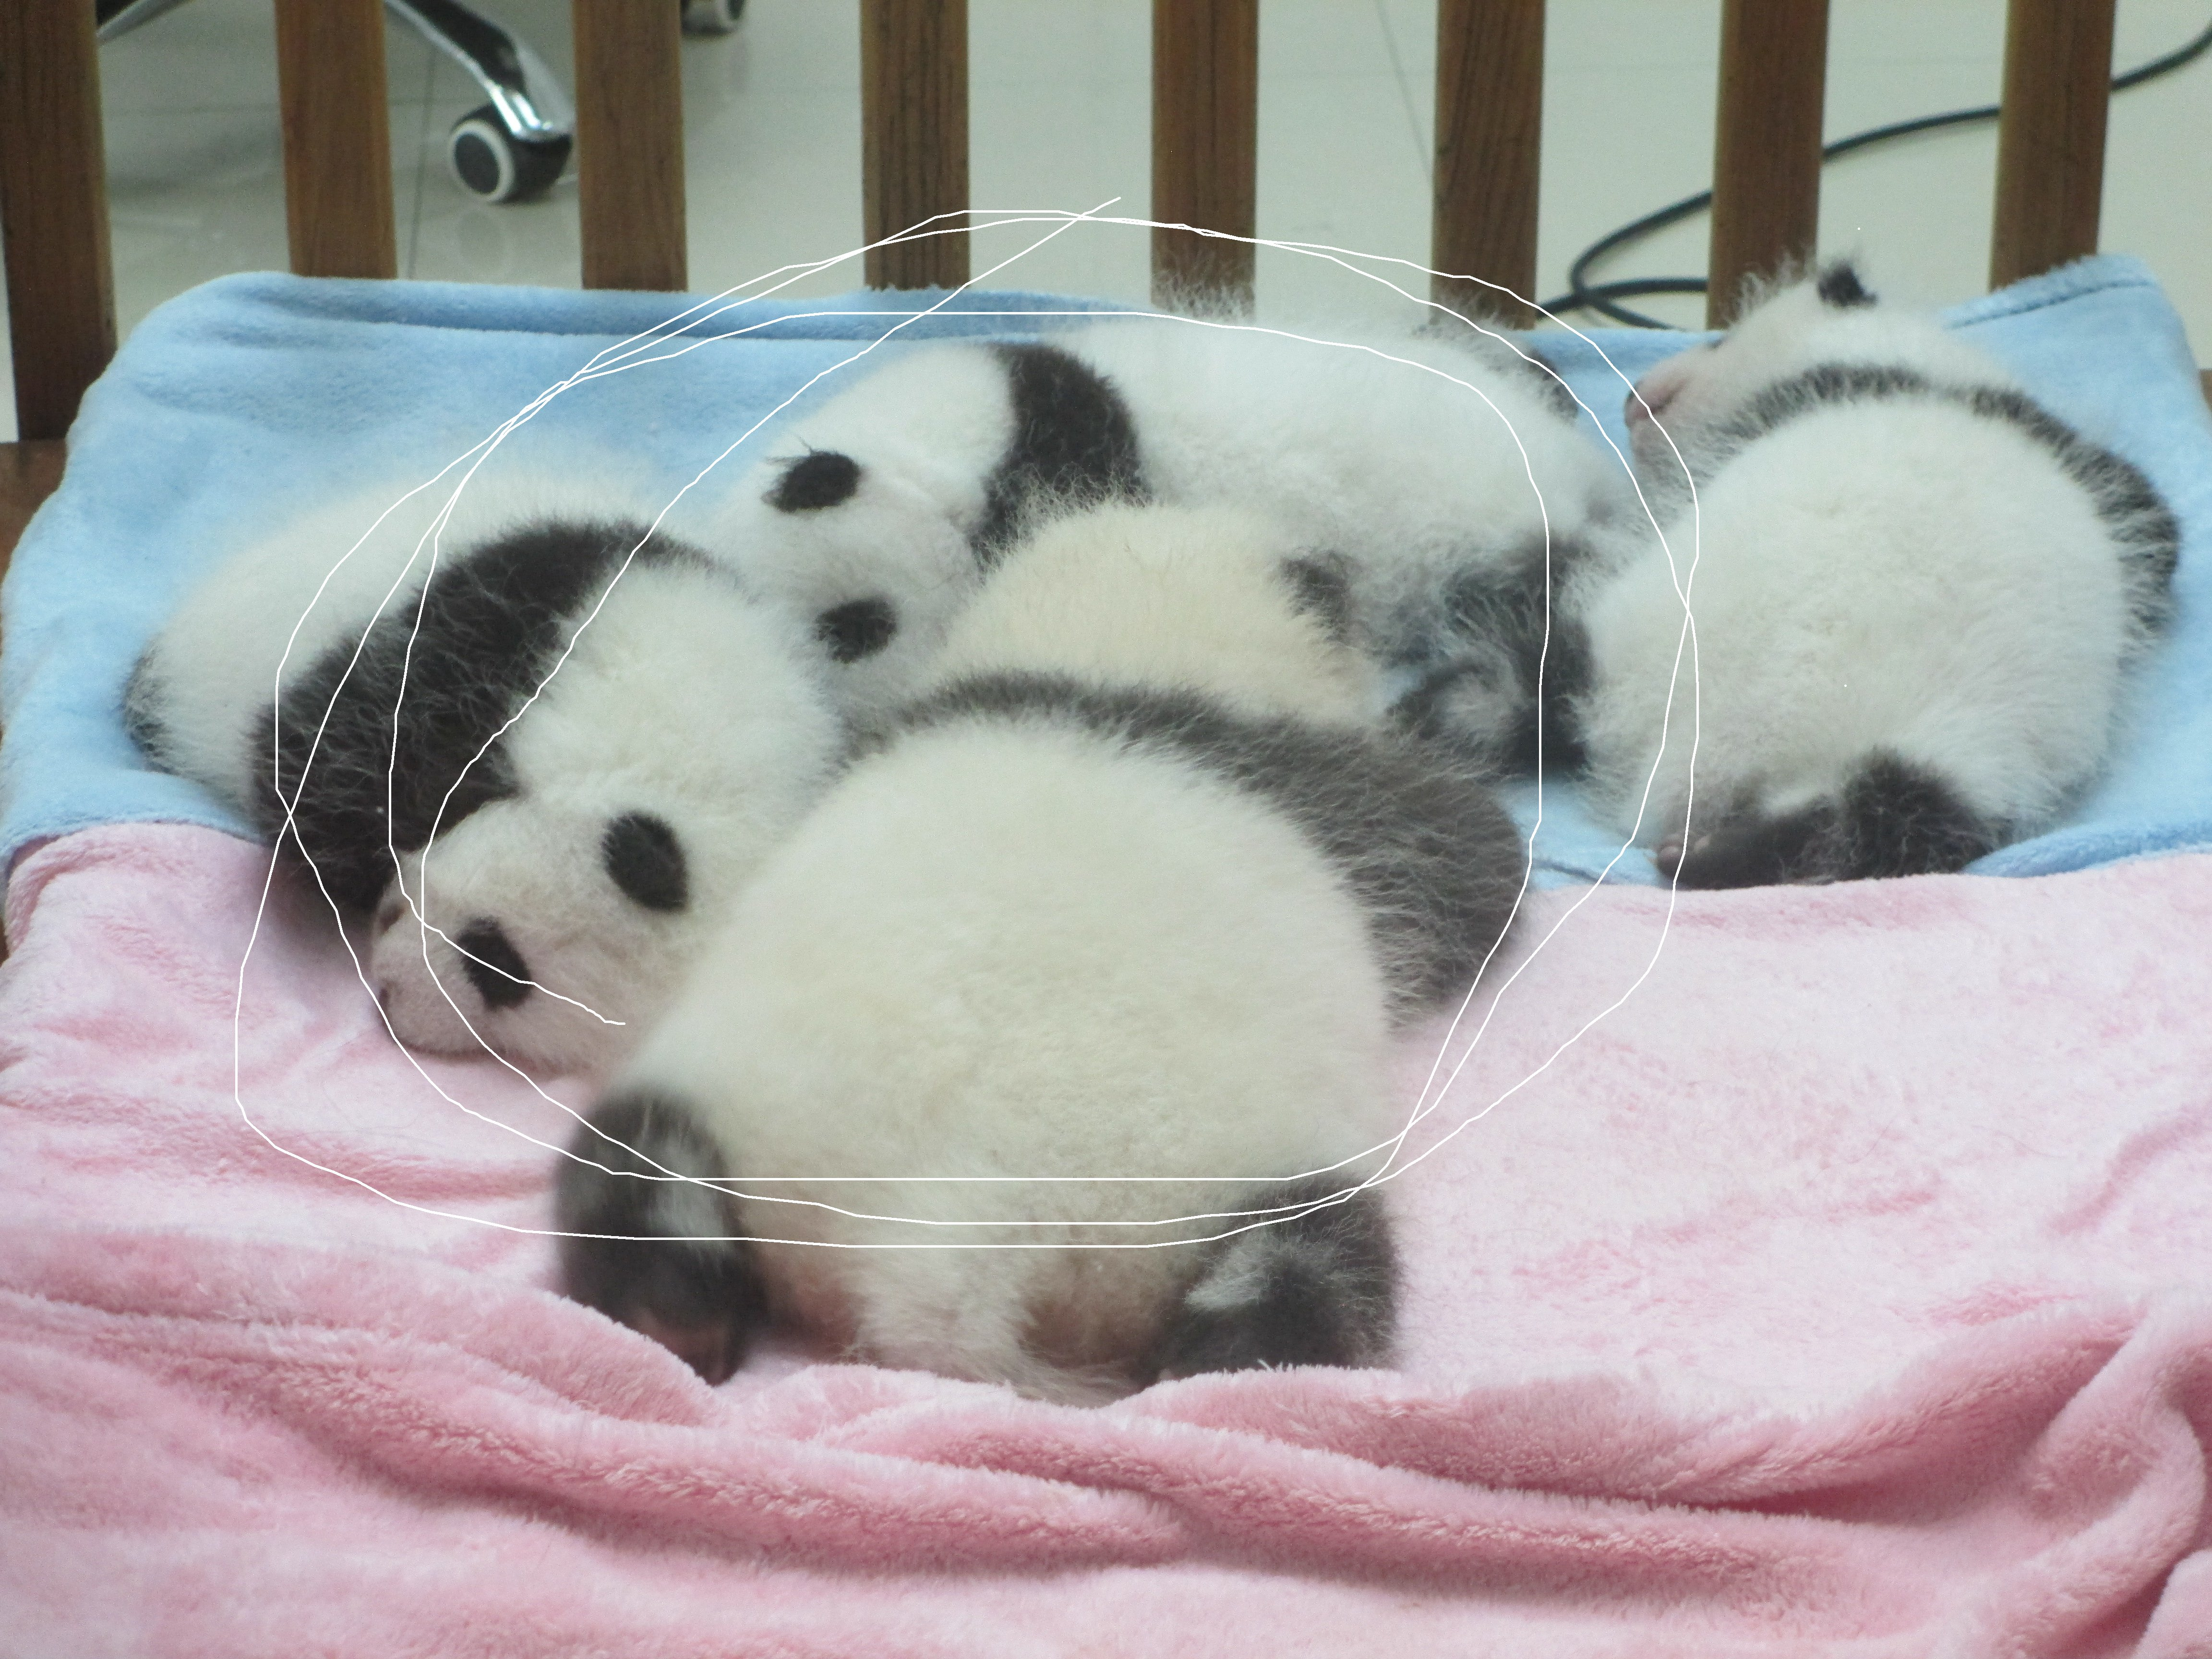
\includegraphics[width = .55\textwidth]{../figures/panda_puppies_v1}
    \end{overprint}

    \begin{alertblock}{An alertblock}
        \begin{itemize}
            \pause
            \item Pandas are furry.
                  \pause
            \item And they are nice !
        \end{itemize}
    \end{alertblock}
\end{frame}




\end{document}